% begin module cycloid-arc-length-ex5
\begin{frame}
\begin{example}
\begin{columns}[c]
\column{.4\textwidth}
\psset{xunit=0.6cm, yunit=0.6cm}
\begin{pspicture}(-0.9, -0.9)(6.8,2.6)
\tiny
\fcAxesStandard{-0.8}{-0.65}{6.8}{2.4}
\fcYTickWithLabel{2}{$2 r$}
\fcXTickWithLabel{6.28319}{$2\pi r$}
%Calculator input: plotCurve{}(- \sin{}t+t, - \cos{}t+1, 0, 2 \pi)
\parametricplot[linecolor=\fcColorGraph, plotpoints=1000]{0}{6.28319}{t t 57.29578 mul sin -1 mul add 1 t 57.29578 mul cos -1 mul add }
\end{pspicture}
%\ 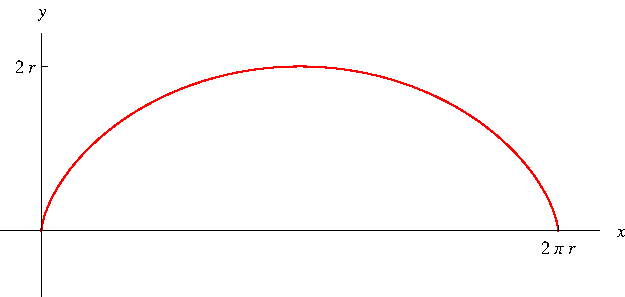
\includegraphics[height=2.2cm]{parametric-curves/pictures/11-02-ex5.pdf}%
\column{.6\textwidth}
Find the length of one arch of the cycloid
\[
\alertNoH{ 3-4}{x = r(\theta - \sin \theta )}, \quad  \alertNoH{ 5-6}{y = r(1-\cos \theta )}.%
\]
\uncover<2->{%
The first arch is \alertNoH{ 2,12}{$0\leq \theta \leq 2\pi$}.
}%
\end{columns}
\abovedisplayskip=0pt
\belowdisplayskip=0pt
\[
\uncover<2->{%
L = \int_{\alertNoH{ 2}{0}}^{\alertNoH{ 2}{2\pi}}\sqrt{\left( \alertNoH{ 3-4}{\frac{\diff x}{\diff \theta}}\right)^2+\left( \alertNoH{ 5-6}{\frac{\diff y}{\diff \theta}}\right)^2} \diff \theta%
}%
\uncover<3->{%
 = \int_0^{2\pi}\sqrt{\left( \alertNoH{ 3-4}{\uncover<4->{r(1-\cos \theta )}}\right)^2+\left( \alertNoH{ 5-6}{\uncover<6->{r\sin \theta}}\right)^2} \diff \theta%
}%
\]
\abovedisplayskip=0pt
\belowdisplayskip=0pt
\[
\uncover<7->{%
 = \int_0^{2\pi} \sqrt{r^2(1 - 2\cos \theta + \cos^2\theta + \sin^2\theta)}\diff \theta%
}%
\uncover<8->{%
 = r \int_0^{2\pi} \sqrt{2(1 - \cos \theta)}\diff \theta%
}%
\]
\uncover<9->{%
Use the identity \alertNoH{ 10}{$\sin^2 x = \frac{1}{2}(1-\cos 2x)$}.  %
}%
\uncover<10->{%
Then %
}%
\abovedisplayskip=0pt
\belowdisplayskip=0pt
\[
\uncover<9->{%
\sqrt{\alertNoH{ 10}{2(1-\cos \theta )}}%
}%
\uncover<10->{%
 = \sqrt{\alertNoH{ 10}{4\sin^2 (\theta /2) }}%
}%
\uncover<11->{%
 = 2\alertNoH{ 12}{|}\sin (\theta /2)\alertNoH{ 12}{|}%
}%
\uncover<12->{%
 = 2\sin (\theta /2)%
}%
\]
\abovedisplayskip=0pt
\belowdisplayskip=0pt
\[
\uncover<13->{%
L = r\int_0^{2\pi}2\sin (\theta /2)\diff \theta%
}%
\uncover<14->{%
 = r\left[ -4\cos (\theta / 2)\right]_0^{2\pi}%
}%
%\uncover<15->{%
% = r\left( (-4)(-1) - (-4)(1)\right)%
%}%
\uncover<15->{%
 = 8r%
}%
\]
\end{example}
\end{frame}
% end module cycloid-arc-length-ex5
